\section{Feedforward networks and backpropagation}
\label{theory-ff-bp}

\subsection{Structure of feedforward networks}

An artificial neural network is made up of a set of nodes $U = \{u_1,
\ldots, u_n\}$. Any two nodes $u_i$ and $u_j$ may be connected by a
directed arc, which has an associated real-valued weight $w_{ij} : i,j
\in \{1, \ldots, n\}$. The backpropagation algorithm works with a
particular type of \emph{feedforward} network: in this network
architecture, nodes are organised into layers, and a link from a
node may only connect to a node in a layer strictly above it in the
network. Thus the network is acyclic. An example of a three-layer
feedforward network is shown in figure \ref{fig-ffn}.

\begin{figure}[htb]
  \label{fig-ffn}
  \centerline{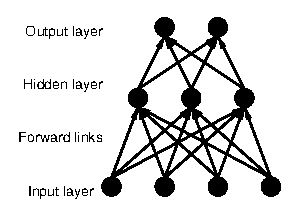
\includegraphics{figs/ffn.eps}}
  \caption{An example of a feedforward network}
\end{figure}

Associated with each node is a number, its \emph{activation}. For
backpropagation networks this is usually a real in the range $[-1,1]$
or $[0,1]$. (My implementation uses $[0,1]$.) The bottom layer in the
network (the one into which no arcs are directed) is termed the
\emph{input layer}; the activations of its nodes are set externally
and form the input of the network. Predictably, the topmost layer is
called the \emph{output layer} and the activations of its nodes will
form the network's output.

For a node $u_i$ not in the input layer, the activation is computed as a
function of the activations of the nodes $u_j$ for which links from
$u_j$ to $u_i$ exist. A weighted sum is taken of the activations, and
a predefined \emph{activation function} $f$ is applied to this sum to give
$u_i$'s activation. The activation $a(u_i)$ is given by

\[ a(u_i) = f(\sum a(w_{ji})u_j) \]

There is one other factor in the activation of a node: its
\emph{bias}. This is simply a constant which is added to the weighted
input sum before the activation function is applied. The easiest and
most common way of implementing bias, and of allowing it to be
modified by training algorithms, is to add an input node with a
constant non-zero activation (usually 1) and make connections from it
to all the hidden and output nodes in the network. The weights of
these connections can then be adjusted by training algorithms just
like any other weights in the network.

Since there is no restriction on the range of the weights and the
activation must be in the range $[0,1]$, the activation function must
map $[-\infty, \infty]$ to $[0,1]$. Additionally, for backpropagation
to work, it must be monotonic and continuous. The most commonly used
function (and the one I use) is the logistic function $f(x) =
\frac{1}{1 + e^{-x}}$.

The process of computing a function using a neural network simply
consists of setting the input activations to the input values, then
successively computing the activations for nodes in subsequent
layers. The activations for the nodes in the final layer form the
output.

\subsection{The backpropagation algorithm}

Backpropagation is an algorithm for adjusting the weights of a
feedforward network in order to make it model a particular function.
It minimizes error by gradient descent: starting from a random point
in weight-space, it ascertains the gradient of the error function and
adjusts the weights in that direction, working towards a minimum.
Unfortunately the minimum is not guaranteed to be global, but it is
nevertheless a powerful algorithm.

In outline, backpropagation works like this:

\begin{enumerate}

\item A training set is assembled, consisting of sample inputs for
  network, with a desired output for each input. The weights of the
  network are initialised to small random values.

\item The network is presented with an input from the training set,
  and a forward-propagation is run to produce output values.

\item The difference is calculated between the actual output values
  and the desired outputs from the training set. These error values are
  propagated backwards through the network, allowing changes in the
  weights of the connections to be calculated.

\item The weights of the connections are altered.

\item Steps 2-4 are repeated until the network models the desired
  function with sufficient accuracy.

\end{enumerate}

In slightly more detail, the backprpagation pass works as follows:

\begin{enumerate}
  
\item Take the derivative of the activation function. If the usual
  logistic function is used, then the identity $f'(x) \equiv
  f(x)(1-f(x))$ can be employed to speed up calculation by using the
  previously computed activations.
  
\item Associate with each node $u_i$ a real number $\delta_i$.
  
\item For each node $u_i$ in the output layer, calculate $\delta_i$ by
  $\delta_i = (C_i - a_i)f'(S_i)$, where $C_i$ is the correct target
  activation for that node, and $S_i$ is the weighted sum used as
  input to the activation function (so actually $\delta_i = (C_i -
  a_i)a_i(1-a_i)$).
  
\item Now move backwards through the network's hidden layers. For each
  node compute $\delta_i = (\sum_j w_{ij}\delta_j)f'(S_i)$, where the
  $j$ range over all the nodes to which forward connections run from
  $i$. Since each $\delta_i$ value only depends on those of the nodes
  in front of it in the network, they can all be computed consistently
  in a single backward pass.

\item Finally, update each weight $w_ij$ with the new value $w_ij +
  \rho \delta_j a_i$. $\rho$ is the learning rate, usually in the
  range 0--1 (see below).

\end{enumerate}

There are numerous variations of the algorithm, and several tunable
parameters which affect its performance. Some of the main variations,
most of which were incorporated into my simulation, are:

\begin{itemize}

\item The actual layout of the network. The number of input and output
  nodes is largely determined by the function which the network is
  being trained to compute, although in this project there is
  considerable choice as to how the inputs and outputs should be
  encoded (see Section \ref{impl-coupling}). The number of hidden
  nodes, however, is an important tunable parameter: too few will
  result in the network being unable to model the desired function,
  and too many will make learning slow and unreliable.
  
  The number of layers is another tunable parameter, but I have kept
  it at three (four including the context nodes) for this project.
  
\item The distribution of the initial random weights, which can have a
  significant effect on the solution which the network converges to.
  
\item A \emph{momentum} parameter can be added to the direction of
  gradient descent, allowing the algorithm to pick up speed if it
  makes many consecutive changes in the same direction. This can speed
  up learning significantly, but can also lead to minima being missed.
  
\item The \emph{learning rate} is a fixed factor governing how much
  the weights are adjusted at each step. Lower values give slower but
  more reliable convergence.
  
\item Instead of updating the weights at each iteration (this is known
  as \emph{stochastic} update), the $\delta_i$ values can be
  accumulated over many iterations, or over the whole training set,
  and only applied at the end (\emph{batch} update).\label{theory-bp-batch}

\end{itemize}
